% CSE 521S Final Report
% A Parking Guidance and Information System for TinyOS
% By Matthew Lindsay, Patrick McBryde, Michael Schultz

\documentclass{acm_proc}
\usepackage{hyperref}
\usepackage{url}
\usepackage{graphicx}

\begin{document}

\title{A Parking Guidance and Information System for TinyOS}
\subtitle{CSE 521S Final Report}

\numberofauthors{3}
\author{
\alignauthor Matthew Lindsay\\
% 2nd. author
\alignauthor Patrick McBryde\\
% 3rd. author
\alignauthor Michael Schultz\\
\and
\affaddr{Washington University in Saint Louis}\\
}

\maketitle

\begin{abstract}
The Internet, in its current form, provides up to the minute updates on
traffic conditions and can provide motorists with detailed mapping and
directions for nearly any destination.
However, once the driver arrives at their destination, they must wander and
search for a parking space, wasting fuel and time, as well as causing
traffic buildups and unnecessary expulsion of greenhouse gasses.
By introducing Wireless Sensor Networks (WSN) into the process, drivers can
be provided with up to the minute updates about parking at a frequency and
cost lower than current implementations.
Currently, expensive induction loops or other, more permanent systems must
be installed, typically only at the entrance and exit to a parking
structure.
	
``Intelligent Transportation Systems'' (ITS) are a mix of systems that
gather various data metrics from transportation areas (parking lots,
streets, alleyways, etc.), aggregate this data together, and present
coherent information to the end-users of the system.
Orchestrating such a system presents several challenges at each level.
How do you gather the data and at what granularity?
Where does the data go once gathered and can it be useful to anyone?
If it can be useful, how can it be presented to end-users to provide
accurate and simple-to-interpret content?
This paper presents and explains our decisions in developing a ``Parking
Guidance and Information'' (PGI) system for TinyOS.
\end{abstract}

\section{Introduction}

Driving to new destinations always brings some level of stress and
uncertainty.
Where am I going, what do the roads and intersections look like, what side
of the road is the place on, where do I park?
These are all questions that dart through the brain when beginning to think
about going some place new.
Luckily, maps bring us the answer or at least a partial answer to some of
those questions.
In the past decade there has been huge growth of web-based mapping
technology to help answer these questions even more fully.
For example, Google Maps allows you to get directions from point A to point
B, and in the past 5 years has introduced Street
View~\cite{vincent:streetview} to their interface.
Street View allows a user to view the roads they will be travelling on from
an in-car perspective.
This removes much of the uncertainty when driving, leading to less
confusion and a better experience (and potentially fewer accidents).

However, there is still that can be done.
Even after you've arrived at your destination you must find where to park.
This can also be quite a hassle, as you are unfamiliar with the area and
during peak hours there may not be a parking space in near proximity.
To help in this matter, Parking Guidance and Information Systems (PGIS)
allow drivers to quickly evaluate where best to go to find parking
efficiently~\cite{sakai:pgi-toyota}.
Traditional PGI Systems simply count the number of cars that enter and exit
a designated area and display the number of spots available in that area to
the driver.
These systems are imprecise, costly, and can't be integrated with other
technologies.

This paper presents our experiences building a parking guidance and
information system using the TelosB/TinyOS platform.
By using motes, it opens the possibility of deploying a single sensor for
each available parking space allowing for much more detailed information
about a parking lot as a whole.
Moreover, with proper sheltering, these sensors can be mounted on the
surface of a parking lot instead of cutting into the lot and installing an
inductive loop to detect vehicle presence.
We also take advantage of the wireless multi-hop routing abilities of
TinyOS-based motes to avoid wiring and enable a heterogeneous mix of
sensors to keep track of parking spot availability and usage data.
Combining these aspects gives a system that can be more precise, lower
cost, and more easily integrated with future technologies.

The remainder of this paper is as follows.
Section~\ref{sec:goals} defines the goals of this project more fully.
Section~\ref{sec:design} presents and explains the high-level architecture
of our PGI System and details the hardware and software used during the
course of this project.
Section~\ref{sec:experiment} talks about how we convinced ourselves that
the system worked correctly and, if we have more resources, could scale up
as needed.
Sections~\ref{sec:related} and~\ref{sec:lessons} give an overview of
related works and lessons we learned during this project.
Finally, Section~\ref{sec:conclusions} concludes this paper with a
discussion of potential future work for this project.

\section{Goals}\label{sec:goals}

Since we believe other solutions to PGI Systems do not represent what
modern technology is capable of, our goals for this project are to build a
PGI System that can be easily deployed at a low-cost, aggregates the data
at a single location, and integrates with user-facing technology to provide
a rich experience.
In short, we plan to answer the following questions:
\begin{itemize}
	\item How do you gather parking data and at what granularity?
	\item Where does the data go once gathered and can it be useful to
	anyone?
	\item How can it be presented to end-users to provide accurate and
	simple-to-interpret content?
\end{itemize}

Our goals for the hardware involve prototyping a low cost, wireless system
which can function with a heterogeneous sensor suite.
This will be accomplished by using sensors with generic connection ports,
allowing for customizing the system to different sensor methods with ease.
Also, using
the built in sensors on the motes, we plan to provide drivers with more
advanced feedback than is traditional in parking structures, such as
headlight detection.
Lastly, our project will be adaptable for any current parking structure.
Therefore, it must make use of the wireless capabilities of the mote
platform, reducing the installation cost by negating the need for expensive
wiring.

Once our system has been installed, we plan to aggregate the data at a base
station, located within the parking structure, which handles interactions
between the WSN and the cloud.
Communication between the base station and the network will rely upon
Collection Tree Protocol (CTP), a robust method of point-to-sink wireless
communication.
Our base station then communicates with a computer via serial port, which
forwards the data to the cloud.

\section{Design}\label{sec:design}

\begin{figure}
    \begin{center}
		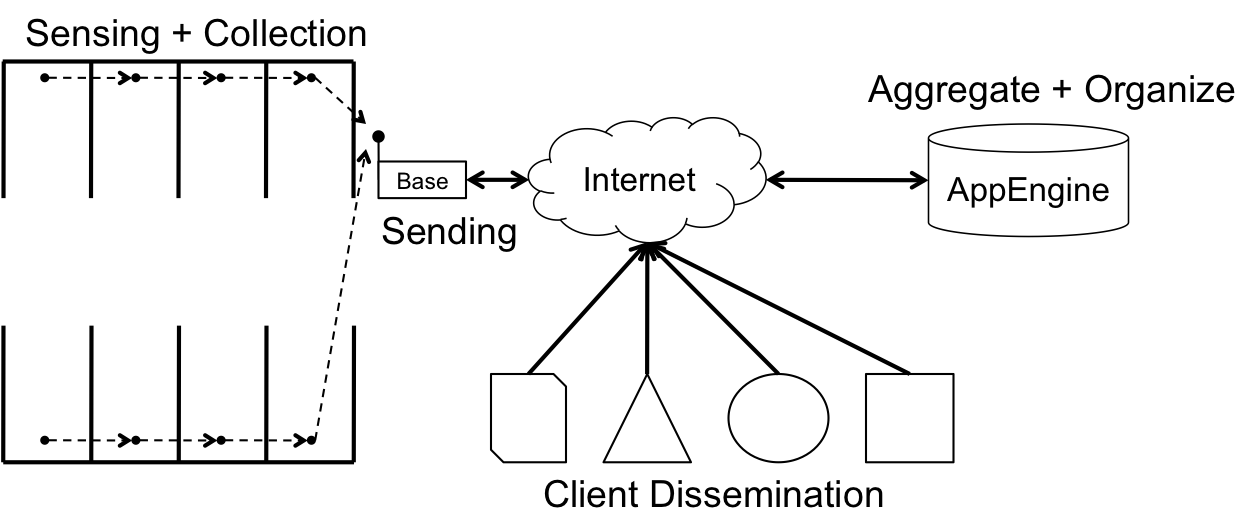
\includegraphics[width=\columnwidth]{figures/high-level}
	\end{center}
	\caption{High-level view of our PGI System. A base station at the lot
	sends data over the Internet to our aggregator, which end-users can
	query.}
	\label{fig:high-level}
\end{figure}

Figure~\ref{fig:high-level} shows a high-level view of the infrastructure
of our PGI System.
Our system begins with a parking lot (left side of
Figure~\ref{fig:high-level}), each space in this lot is equipped with a
sensor built on the TelosB/TinyOS platform.
Data is collected at a per-lot base station, which then sends the data over
the Internet to our backend.
When our backend receives the data it updates and logs the changes to the
data store and organizes the lot information.
Once the data is stored, clients are able to query the backend and get
up-to-date information about a specific lot and lots in the vicinity.

Building this system requires a fair amount of hardware and software
knowledge and is described below.

\subsection{Hardware}
When choosing the hardware for our PGI system we had specific goals in mind.  The system would need to be low cost, reliable, power efficient, and easily customized to meet the needs of the specific structure/lot.  

We believe most of our potential business would come from upgrading existing parking structures versus that of new construction.  This is why we believe the need for the system to be easily customized is the most important requirement for a successful adoption by the parking industry.  When adding a system such as this it is typically the installation cost that are prohibitive vs the devices themselves 

By supporting many different sensor types and configurations for existing construction we are providing new construction many options as well.

\subsubsection{Parking Space Monitors}

The Parking Space Monitors need to be able to do more than just determine if a vehicle is present in a parking space.  They need to be able to run on a set of batteries for an extended period of time, support multiple sensor types and interfaces, wireless transmit relevant data to a base-station.  For all these reasons we chose the TelosB wireless sensor module as the base to our Parking Space Monitors.  The TelosBs provide a multitude of features and sensor and still manages to support.

\begin{figure}[h]
    \begin{center}
		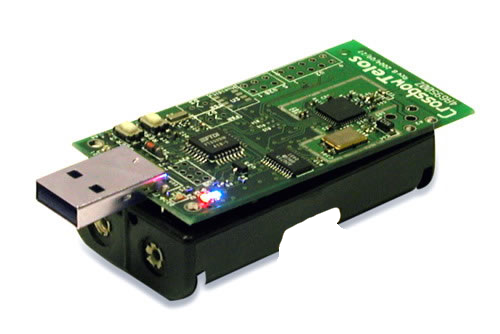
\includegraphics[width=\columnwidth]{figures/telosb}
	\end{center}
	\caption{TelosB.}
	\label{fig:telosb}
\end{figure}

The TelosB is an ultra low power IEEE 802.15.4 compliant wireless sensor module.  More about the TelosB.

By choosing the TelosB we have many different options to attach sensors with
The parking space monitors are the 

There are many different types of sensors that we could have been used to monitor if a parking space is occupied or vacant.  These include infrared range finders, magnetic

We chose to use ultra sonic 

\begin{figure}[h]
    \begin{center}
		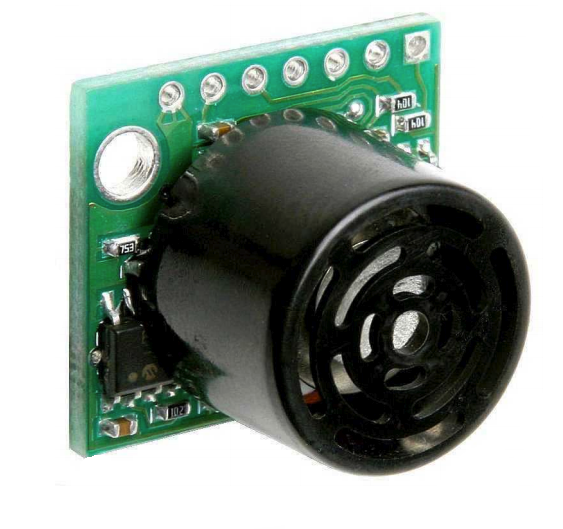
\includegraphics[width=\columnwidth]{figures/range_finder}
	\end{center}
	\caption{LV-MaxSonar-EZ1.}
	\label{fig:range_finder}
\end{figure}

To actual

LV-MaxSonar-EZ1 - Ultrasonic Rangefinder
Supply voltage 2.5V to 5.5V
Detects objects from 6 inches out to 254 inches with 1 inch resolution (0-6 inches range as 6 inches)
Output formats include pulse width, analog voltage, and serial digital

\subsubsection{Base-Station}
Following with our theme of low cost we tried to keep the requirements of the base-station to a minimum as well.  The base-station will support multiple 

The base-station has two key roles.  First

In order to reliably and cost effectively  monitor the status of individual parking spaces in a lot or garage we need reliable, low cost hardware

The TelosB mote was chosen to monitor 

This should cover the physical hardware we used in building this.
Including (but not limited to):

- TelosB motes (listing any relevant specifications, why we used TelosB
 and not something else) \cite{xbow:telosb-datasheet}.

- External sensor we used, specifications for that, more detail than
 TelosB since the reader will be less familiar with it, why we used that.

At least one pictures of the telosb, the sensors, or the telosb with sensor
attached.

\subsection{Collection Software}

\subsubsection{Parking Space Monitors}

The Parking Space Monitors are powered by TinyOS.  We chose TinyOS because it fully supports the TelosB and provides many features that rapidly speed-up development and 

One of out key design goals was wireless reliability.  We need to ensure that packets containing sensor details always make it back to the base-station for processing.  This can be very difficult in dynamic environment such as a parking structure.  


CTP stuff~\cite{tep119:collection}.

\subsubsection{Base-Station}

The base-station has multiple function.  It is responsible for configuring the Parking Space Monitors, ensuring the Parking Space Monitors are

The base station collects sensor reading from the parking space monitors and determines what data is import

Collects sensor data.

Determines what data is important

Since the base-station has a TelosB.


\subsection{Aggregation Software}

Data leaving the base station of a parking lot is directed over then
Internet to our aggregation software hosted on Google's
AppEngine~\cite{google:appengine}.
For this project, we decided the AppEngine environment was an appropriate
choice for several reasons:
\begin{itemize}
	\item The service is free for light usage (testing and development).
	\item It provides a Python programming environment.
	\item Most importantly, it is designed to scale up with ease
	transparently with large datasets.
\end{itemize}

The nature of our project is to have one sensor per parking space in a
parking lot for every parking lot.
This implies that over time our backend must be able to accept, store, and
recall large amounts of current and historical data.
We could have sunk our resources into using a traditional server model for
the purposes of a prototype, however if the project were to start scaling
up great amounts we would start running into resource barriers.
Google's AppEngine is designed to scale with demand, this is largely due to
their use of a datastore built on top of Bigtable~\cite{google:bigtable}.
Though transparent to users of our system, this non-SQL based datastore
forced a few notable differences from a SQL based datastore.

First, while queries appear to be SQL, they are actually ``GQL,'' a
SQL-like language.
In general this does not bring any problems, but because of the
organization of the datastore imprecise queries are not acceptable.
You must know the data you are looking for.
You cannot simple SELECT one or two columns from the datastore, rather you
must get all the columns or a unique key identifier that matches the query.

Second, its harder to perform proximity searches with the datastore because
there is not concept of ``similar'' or ``like'' queries, you either know
the data or don't know the data.
However, with the help of the geomodel API~\cite{geomodel} we are able to
use geohashing to perform proximity searches on the datastore.
This is useful to locate nearby parking lots, allowing the end-user to
identify other potential parking areas.

With an understanding of the underlying technology, we are able to present
an easy to use API.

\subsubsection{A RESTful API}

REpresentational State Transfer (REST) is an abstract model for building
large-scale web services~\cite{pautasso:restful}.
The principles of a RESTful architecture are an identification of resources
through a URI, a ``pure'' HTTP interface, and self-contained hyperlinks.
In this section we describe how we achieved these principles.

Our URI scheme is straight-forward.
Each lot is given a unique identification consisting of alphanumerics and
the underscore (\_) character.
When attempting to access a specific lot, that identifier is part of the
URI (i.e.,
\texttt{http://<host>/lot/wustl\_millbrook/}
identifies the Milbrook lot on Washington University's campus).

\begin{figure}
    \begin{verbatim}
[
  {
    "space_id": 8,
    "is_empty": false,
    "magnet": 218,
    "sonar": 114
  },
  ...
]
\end{verbatim}
	\caption{Client to server JSON data.}
	\label{fig:clientserverjson}
\end{figure}

Any request concerning this lot must go through its URI.
Requests use one of the HTTP verbs of \texttt{GET}, \texttt{PUT}, or
\texttt{POST}.
A \texttt{GET} request simply returns the information for the requested URI
in either the HTML or JSON format.
A \texttt{PUT} request attempts to store updated status information to the
lot.
This request contains the list of parking spaces to update, their
identification and status, as well as any associated meta-information that
should be put in the datastore, an example of this can be seen in
Figure~\ref{fig:clientserverjson}.
Finally, a \texttt{POST} request handles the creation of new parking lots.

With the API in place, we are able to create rich applications with ease
for expansion and integration into other software.
As a demonstration, we build up a web-based frontend in the next section
that takes advantage of our API.

\subsubsection{Frontend}

\begin{figure}
    \begin{verbatim}
{
  "lot_id": "wustl_snowway",
  "geo_pt": "38.650233,-90.313529",
  "timestamp": 1291946695.0
  "spaces":
  [
    {
      "space_id": "4",
      "is_empty": false,
      "timestamp": 1291946695.0,
      "extra_info": "sonar:55;magnet:201;"
    },
    ...
  ]
}
\end{verbatim}
	\caption{Server to client JSON data.}
	\label{fig:serverclientjson}
\end{figure}

As mentioned above, a \texttt{GET} request on the parking lot identifier
will result in either a HTML or JSON response.
An example of the JSON response can be seen in
Figure~\ref{fig:serverclientjson}.
The response provides enough information to a client application to
identify the name of the lot, its location, the time of the most recent
activity, and the list of spaces.
Each space has a unique identifier, the status of that spot (full or
empty), the time it was last updated, and any additional information about
that spot (likely to be sensor readings at the last report).
A client can combine this information with a virtual representation of the
lot's topography, then keep that representation up-to-date by periodically
querying the server for new information.

For our project, we've also built an HTML interface for viewing the
information on a lot.
Once a lot is selected by the user, our interface provides a map of the
area surrounding the lot with markers indicating other lots in a two mile
radius.
It also displays a ``health'' indicator giving an approximate empty-to-full
ratio, as well as a list of spaces that are filled and how long they've
been filled.

\begin{figure}
    \begin{center}
		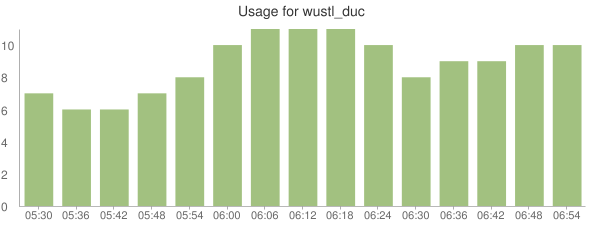
\includegraphics[width=\columnwidth]{figures/fullness-chart}
	\end{center}
	\caption{Example of a usage chart for the 5:30am--7:00am time slot.}
	\label{fig:fullness-chart}
\end{figure}

Additionally, by keeping a log of changes to a lot on the backend, we are
able to provide a chart to indicate the average fullness of a lot over a
time frame.
For example, Figure~\ref{fig:fullness-chart} shows the average fullness of
the ``DUC'' lot from 5:30am until 7:00am.
At the 6:06am time slot there are 11 spaces being used, however only 20
minutes earlier only 6 spaces are being used.
Having access to this information would allow a daily commuter, or one time
visitor, discover that by arriving only 20 minutes earlier they would have
a much greater chance of easily finding a parking space.

\section{Experiment}\label{sec:experiment}

Since our system was split into two major components, we were able to test
both somewhat independently. 
The first component included physically sensing the vehicle and relaying
the data to the backend.
The second component involved testing the backend works for extended
periods of time and correctly logs/recalls historical data.

\subsection{Sensing and Sending}

Sensing and sending from the Parking Space Monitors to the base-station to the 

\begin{figure}[h]
    \begin{center}
		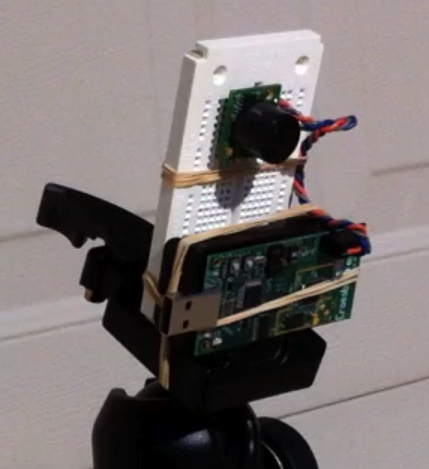
\includegraphics[width=\columnwidth]{figures/parking_sensor}
	\end{center}
	\caption{Parking Space Monitor on tripod for testing.}
	\label{fig:parking_sensor}
\end{figure}

A great deal of testing was performed on the sensing and sending portion of this project.  Figure~\ref{fig:parking_sensor}  shows a Parking Space Monitor mounted on a tripod 

It was through this testing that we found the issues with the range of our Parking Space Monitors.  The EZ1 claims to support a distance up to 254-inches, however we were only able to detect a vehicle   The EZ1 range finder will support a supply voltage of 2.5V - 5.5V.  The EZ1 is powered by the TelosB analog supply of ~3.1V.  

\subsection{Backend and Frontend}

Discussion of how the simulator tested the backend and any problems that
arose from it.
% Couldn't really test large scale deployment of sensor backend since we
% had limited resources with respect to actual motes, funds to purchase
% sonar sensors, building containers to house the sensors overnight, and
% the ability to gather data over an extended period of time.

\section{Related Work}\label{sec:related}

There are other proposals and existing systems for parking guidance and
information, here we'll discuss and differentiate ourselves from these
systems.

Signal-Park, uses sonar sensors above each parking spot to detect the
presence of a vehicle~\cite{pgi:signal-park}.
Approximately three times per second, the sensor is queried to determine
vehicle presences and updates a central computer.
This system uses serial lines to connect each sensor with the central
computer, leading to more costly deploy.
It also appears to be limited to the parking lot that it is deployed in and
lacks the ability to aggregate the information for others to benefit.
It would certainly be possible to improve the connectivity of this system
to integrate with our back-end aggregation system to take advantage of
existing installations.

Streetline, is a startup in the San Francisco area that similarly uses a
wireless mesh network to link all the sensors
together~\cite{pgi:streetline}.
The Streetline system has recently (Summer 2010) begun to roll out sensors
and upgraded meters for select areas in the San Francisco
area~\cite{wired:streetline, sfpark}.
This system uses surface (and sub-surface) sensor mounts that contain a
wireless transmitter and a magnetometer for vehicle detection.
Status is sent to a central aggregation server where users can see the
status of street parking via their web browser, text message, or smart
phone; it also allows municipal workers to identify vehicles that have not
paid fully.
Presuming the Streetline trial is successful and the system expands, our
system and their system should be able to integrate with little effort and
could be seen as competitors.
We view this a positive, as it demonstrates that our project is a useful
idea with potential buyers available.

There has also been a proposal to use existing security cameras with a view
of a parking lot to detect vehicular presence~\cite{lin:vision-parking}.
The results of their experiment, while decent for their scenario, seem
unlikely to generalize to other systems.
While it may be true that some lots have existing surveillance cameras, the
paper also observes that cameras should be mounted higher for a more
consistent and complete view of the lot.
This goes against their principal of using existing cameras for the
information, since additional cameras would have to be mounted to perform
correctly (moving security cameras further from the observation area is
probably not acceptable to the security officers).

\section{Lessons Learned}\label{sec:lessons}

If we were to pursue this project into the future we would probably modify the design of the sensor placement.

Anything we would have done differently if we were to pursue this project
in more detail again.

\section{Conclusions and Future Work}\label{sec:conclusions}

Conclusions from this project.

\bibliographystyle{abbrv}
\bibliography{report}

\end{document}
